% Options for packages loaded elsewhere
\PassOptionsToPackage{unicode}{hyperref}
\PassOptionsToPackage{hyphens}{url}
%
\documentclass[
]{article}
\usepackage{amsmath,amssymb}
\usepackage{lmodern}
\usepackage{ifxetex,ifluatex}
\ifnum 0\ifxetex 1\fi\ifluatex 1\fi=0 % if pdftex
  \usepackage[T1]{fontenc}
  \usepackage[utf8]{inputenc}
  \usepackage{textcomp} % provide euro and other symbols
\else % if luatex or xetex
  \usepackage{unicode-math}
  \defaultfontfeatures{Scale=MatchLowercase}
  \defaultfontfeatures[\rmfamily]{Ligatures=TeX,Scale=1}
\fi
% Use upquote if available, for straight quotes in verbatim environments
\IfFileExists{upquote.sty}{\usepackage{upquote}}{}
\IfFileExists{microtype.sty}{% use microtype if available
  \usepackage[]{microtype}
  \UseMicrotypeSet[protrusion]{basicmath} % disable protrusion for tt fonts
}{}
\makeatletter
\@ifundefined{KOMAClassName}{% if non-KOMA class
  \IfFileExists{parskip.sty}{%
    \usepackage{parskip}
  }{% else
    \setlength{\parindent}{0pt}
    \setlength{\parskip}{6pt plus 2pt minus 1pt}}
}{% if KOMA class
  \KOMAoptions{parskip=half}}
\makeatother
\usepackage{xcolor}
\IfFileExists{xurl.sty}{\usepackage{xurl}}{} % add URL line breaks if available
\IfFileExists{bookmark.sty}{\usepackage{bookmark}}{\usepackage{hyperref}}
\hypersetup{
  hidelinks,
  pdfcreator={LaTeX via pandoc}}
\urlstyle{same} % disable monospaced font for URLs
\usepackage[margin=1in]{geometry}
\usepackage{color}
\usepackage{fancyvrb}
\newcommand{\VerbBar}{|}
\newcommand{\VERB}{\Verb[commandchars=\\\{\}]}
\DefineVerbatimEnvironment{Highlighting}{Verbatim}{commandchars=\\\{\}}
% Add ',fontsize=\small' for more characters per line
\usepackage{framed}
\definecolor{shadecolor}{RGB}{248,248,248}
\newenvironment{Shaded}{\begin{snugshade}}{\end{snugshade}}
\newcommand{\AlertTok}[1]{\textcolor[rgb]{0.94,0.16,0.16}{#1}}
\newcommand{\AnnotationTok}[1]{\textcolor[rgb]{0.56,0.35,0.01}{\textbf{\textit{#1}}}}
\newcommand{\AttributeTok}[1]{\textcolor[rgb]{0.77,0.63,0.00}{#1}}
\newcommand{\BaseNTok}[1]{\textcolor[rgb]{0.00,0.00,0.81}{#1}}
\newcommand{\BuiltInTok}[1]{#1}
\newcommand{\CharTok}[1]{\textcolor[rgb]{0.31,0.60,0.02}{#1}}
\newcommand{\CommentTok}[1]{\textcolor[rgb]{0.56,0.35,0.01}{\textit{#1}}}
\newcommand{\CommentVarTok}[1]{\textcolor[rgb]{0.56,0.35,0.01}{\textbf{\textit{#1}}}}
\newcommand{\ConstantTok}[1]{\textcolor[rgb]{0.00,0.00,0.00}{#1}}
\newcommand{\ControlFlowTok}[1]{\textcolor[rgb]{0.13,0.29,0.53}{\textbf{#1}}}
\newcommand{\DataTypeTok}[1]{\textcolor[rgb]{0.13,0.29,0.53}{#1}}
\newcommand{\DecValTok}[1]{\textcolor[rgb]{0.00,0.00,0.81}{#1}}
\newcommand{\DocumentationTok}[1]{\textcolor[rgb]{0.56,0.35,0.01}{\textbf{\textit{#1}}}}
\newcommand{\ErrorTok}[1]{\textcolor[rgb]{0.64,0.00,0.00}{\textbf{#1}}}
\newcommand{\ExtensionTok}[1]{#1}
\newcommand{\FloatTok}[1]{\textcolor[rgb]{0.00,0.00,0.81}{#1}}
\newcommand{\FunctionTok}[1]{\textcolor[rgb]{0.00,0.00,0.00}{#1}}
\newcommand{\ImportTok}[1]{#1}
\newcommand{\InformationTok}[1]{\textcolor[rgb]{0.56,0.35,0.01}{\textbf{\textit{#1}}}}
\newcommand{\KeywordTok}[1]{\textcolor[rgb]{0.13,0.29,0.53}{\textbf{#1}}}
\newcommand{\NormalTok}[1]{#1}
\newcommand{\OperatorTok}[1]{\textcolor[rgb]{0.81,0.36,0.00}{\textbf{#1}}}
\newcommand{\OtherTok}[1]{\textcolor[rgb]{0.56,0.35,0.01}{#1}}
\newcommand{\PreprocessorTok}[1]{\textcolor[rgb]{0.56,0.35,0.01}{\textit{#1}}}
\newcommand{\RegionMarkerTok}[1]{#1}
\newcommand{\SpecialCharTok}[1]{\textcolor[rgb]{0.00,0.00,0.00}{#1}}
\newcommand{\SpecialStringTok}[1]{\textcolor[rgb]{0.31,0.60,0.02}{#1}}
\newcommand{\StringTok}[1]{\textcolor[rgb]{0.31,0.60,0.02}{#1}}
\newcommand{\VariableTok}[1]{\textcolor[rgb]{0.00,0.00,0.00}{#1}}
\newcommand{\VerbatimStringTok}[1]{\textcolor[rgb]{0.31,0.60,0.02}{#1}}
\newcommand{\WarningTok}[1]{\textcolor[rgb]{0.56,0.35,0.01}{\textbf{\textit{#1}}}}
\usepackage{graphicx}
\makeatletter
\def\maxwidth{\ifdim\Gin@nat@width>\linewidth\linewidth\else\Gin@nat@width\fi}
\def\maxheight{\ifdim\Gin@nat@height>\textheight\textheight\else\Gin@nat@height\fi}
\makeatother
% Scale images if necessary, so that they will not overflow the page
% margins by default, and it is still possible to overwrite the defaults
% using explicit options in \includegraphics[width, height, ...]{}
\setkeys{Gin}{width=\maxwidth,height=\maxheight,keepaspectratio}
% Set default figure placement to htbp
\makeatletter
\def\fps@figure{htbp}
\makeatother
\setlength{\emergencystretch}{3em} % prevent overfull lines
\providecommand{\tightlist}{%
  \setlength{\itemsep}{0pt}\setlength{\parskip}{0pt}}
\setcounter{secnumdepth}{-\maxdimen} % remove section numbering
\usepackage{booktabs}
\usepackage{longtable}
\usepackage{array}
\usepackage{multirow}
\usepackage{wrapfig}
\usepackage{float}
\usepackage{colortbl}
\usepackage{pdflscape}
\usepackage{tabu}
\usepackage{threeparttable}
\usepackage{threeparttablex}
\usepackage[normalem]{ulem}
\usepackage{makecell}
\usepackage{xcolor}
\ifluatex
  \usepackage{selnolig}  % disable illegal ligatures
\fi

\author{}
\date{\vspace{-2.5em}}

\begin{document}

\hypertarget{bsscol}{%
\section{bsscol}\label{bsscol}}

bsscol allows for a simple integration of the BSS base colors into
ggplot2 and alike.

\hypertarget{installation}{%
\subsection{installation}\label{installation}}

You can install the released version of bsscol from
\href{https://github.com/qwertzlbry/bsscol}{Github} with:

\begin{Shaded}
\begin{Highlighting}[]
\FunctionTok{library}\NormalTok{(devtools) }\CommentTok{\# install devtool first if not installed}
\FunctionTok{install\_github}\NormalTok{(}\StringTok{"qwertzlbry/bsscol"}\NormalTok{)}
\end{Highlighting}
\end{Shaded}

With a future CRAN approval the package could be installed with:

\begin{Shaded}
\begin{Highlighting}[]
\FunctionTok{install.packages}\NormalTok{(}\StringTok{"bsscol"}\NormalTok{) }\CommentTok{\# currently the installation works only over github}
\end{Highlighting}
\end{Shaded}

In order to run the following examples you'll also need:

\begin{Shaded}
\begin{Highlighting}[]
\FunctionTok{install.packages}\NormalTok{(}\StringTok{"ggplot2"}\NormalTok{)}
\FunctionTok{install.packages}\NormalTok{(}\StringTok{"plotrix"}\NormalTok{)}
\FunctionTok{install.packages}\NormalTok{(}\StringTok{"dplyr"}\NormalTok{)}
\FunctionTok{install.packages}\NormalTok{(}\StringTok{"hues"}\NormalTok{)}
\FunctionTok{install.packages}\NormalTok{(}\StringTok{"DT"}\NormalTok{)}
\end{Highlighting}
\end{Shaded}

\hypertarget{load-packages}{%
\subsection{load packages}\label{load-packages}}

\begin{Shaded}
\begin{Highlighting}[]
\FunctionTok{library}\NormalTok{(bsscol)}
\FunctionTok{library}\NormalTok{(ggplot2)}
\FunctionTok{library}\NormalTok{(plotrix)}
\FunctionTok{library}\NormalTok{(hues)}
\FunctionTok{library}\NormalTok{(dplyr)}
\CommentTok{\#\textgreater{} }
\CommentTok{\#\textgreater{} Attaching package: \textquotesingle{}dplyr\textquotesingle{}}
\CommentTok{\#\textgreater{} The following objects are masked from \textquotesingle{}package:stats\textquotesingle{}:}
\CommentTok{\#\textgreater{} }
\CommentTok{\#\textgreater{}     filter, lag}
\CommentTok{\#\textgreater{} The following objects are masked from \textquotesingle{}package:base\textquotesingle{}:}
\CommentTok{\#\textgreater{} }
\CommentTok{\#\textgreater{}     intersect, setdiff, setequal, union}
\FunctionTok{library}\NormalTok{(kableExtra)}
\CommentTok{\#\textgreater{} }
\CommentTok{\#\textgreater{} Attaching package: \textquotesingle{}kableExtra\textquotesingle{}}
\CommentTok{\#\textgreater{} The following object is masked from \textquotesingle{}package:dplyr\textquotesingle{}:}
\CommentTok{\#\textgreater{} }
\CommentTok{\#\textgreater{}     group\_rows}
\end{Highlighting}
\end{Shaded}

\hypertarget{the-colors}{%
\subsection{the colors}\label{the-colors}}

\begin{Shaded}
\begin{Highlighting}[]
\CommentTok{\# the colors, RGB and hex codes }
\NormalTok{bss\_colors }\OtherTok{\textless{}{-}}\NormalTok{ bss\_colors }\SpecialCharTok{\%\textgreater{}\%} \FunctionTok{arrange}\NormalTok{(col\_pal) }\SpecialCharTok{\%\textgreater{}\%} \FunctionTok{select}\NormalTok{(}\SpecialCharTok{{-}}\NormalTok{colour)}
\NormalTok{bss\_dt }\OtherTok{\textless{}{-}}\NormalTok{ bss\_colors}
\NormalTok{bss\_dt}\SpecialCharTok{$}\NormalTok{hashed\_hex }\OtherTok{=} \FunctionTok{cell\_spec}\NormalTok{(}
\NormalTok{  bss\_dt}\SpecialCharTok{$}\NormalTok{hashed\_hex, }\AttributeTok{color =} \StringTok{"white"}\NormalTok{, }\AttributeTok{align =} \StringTok{"c"}\NormalTok{, }\CommentTok{\#angle = 2, }
  \AttributeTok{background =} \FunctionTok{factor}\NormalTok{(bss\_dt}\SpecialCharTok{$}\NormalTok{excel\_form,bss\_dt}\SpecialCharTok{$}\NormalTok{excel\_form, bss\_dt}\SpecialCharTok{$}\NormalTok{hashed\_hex))}

\FunctionTok{kbl}\NormalTok{(bss\_dt, }\AttributeTok{escape =}\NormalTok{ F) }\SpecialCharTok{\%\textgreater{}\%}
  \FunctionTok{kable\_paper}\NormalTok{(}\StringTok{"striped"}\NormalTok{, }\AttributeTok{full\_width =}\NormalTok{ F)}
\end{Highlighting}
\end{Shaded}

\begin{table}
\centering
\begin{tabular}[t]{l|l|l|l|r|l|r|l|r|l}
\hline
R & G & B & hex & Typ & Full & col_pal & hashed_hex & excel_form & name\\
\hline
255 & 255 & 255 & FFFFFF & 0 & 255,255,255 & 1 & \multicolumn{1}{c}{\cellcolor[HTML]{FFFFFF}{\textcolor{white}{\#FFFFFF}}} & 1 & weiss\\
\hline
242 & 242 & 242 & F2F2F2 & -5 & 242,242,242 & 1 & \multicolumn{1}{c}{\cellcolor[HTML]{F2F2F2}{\textcolor{white}{\#F2F2F2}}} & 11 & NA\\
\hline
217 & 217 & 217 & D9D9D9 & -15 & 217,217,217 & 1 & \multicolumn{1}{c}{\cellcolor[HTML]{D9D9D9}{\textcolor{white}{\#D9D9D9}}} & 21 & NA\\
\hline
191 & 191 & 191 & BFBFBF & -25 & 191,191,191 & 1 & \multicolumn{1}{c}{\cellcolor[HTML]{BFBFBF}{\textcolor{white}{\#BFBFBF}}} & 31 & NA\\
\hline
166 & 166 & 166 & A6A6A6 & -35 & 166,166,166 & 1 & \multicolumn{1}{c}{\cellcolor[HTML]{A6A6A6}{\textcolor{white}{\#A6A6A6}}} & 41 & NA\\
\hline
128 & 128 & 128 & 808080 & -50 & 128,128,128 & 1 & \multicolumn{1}{c}{\cellcolor[HTML]{808080}{\textcolor{white}{\#808080}}} & 51 & NA\\
\hline
0 & 0 & 0 & 000000 & 0 & 0,0,0 & 2 & \multicolumn{1}{c}{\cellcolor[HTML]{000000}{\textcolor{white}{\#000000}}} & 2 & schwarz\\
\hline
128 & 128 & 128 & 808080 & 50 & 128,128,128 & 2 & \multicolumn{1}{c}{\cellcolor[HTML]{808080}{\textcolor{white}{\#808080}}} & 12 & NA\\
\hline
89 & 89 & 89 & 595959 & 35 & 89,89,89 & 2 & \multicolumn{1}{c}{\cellcolor[HTML]{595959}{\textcolor{white}{\#595959}}} & 22 & NA\\
\hline
64 & 64 & 64 & 404040 & 25 & 64,64,64 & 2 & \multicolumn{1}{c}{\cellcolor[HTML]{404040}{\textcolor{white}{\#404040}}} & 32 & NA\\
\hline
38 & 38 & 38 & 262626 & 15 & 38,38,38 & 2 & \multicolumn{1}{c}{\cellcolor[HTML]{262626}{\textcolor{white}{\#262626}}} & 42 & NA\\
\hline
13 & 13 & 13 & 0D0D0D & 5 & 13,13,13 & 2 & \multicolumn{1}{c}{\cellcolor[HTML]{0D0D0D}{\textcolor{white}{\#0D0D0D}}} & 52 & NA\\
\hline
242 & 242 & 242 & F2F2F2 & 0 & 242,242,242 & 3 & \multicolumn{1}{c}{\cellcolor[HTML]{F2F2F2}{\textcolor{white}{\#F2F2F2}}} & 3 & hellgrau1\\
\hline
218 & 218 & 218 & DADADA & -10 & 218,218,218 & 3 & \multicolumn{1}{c}{\cellcolor[HTML]{DADADA}{\textcolor{white}{\#DADADA}}} & 13 & NA\\
\hline
182 & 182 & 182 & B6B6B6 & -25 & 182,182,182 & 3 & \multicolumn{1}{c}{\cellcolor[HTML]{B6B6B6}{\textcolor{white}{\#B6B6B6}}} & 23 & NA\\
\hline
121 & 121 & 121 & 797979 & -50 & 121,121,121 & 3 & \multicolumn{1}{c}{\cellcolor[HTML]{797979}{\textcolor{white}{\#797979}}} & 33 & NA\\
\hline
61 & 61 & 61 & 3D3D3D & -75 & 61,61,61 & 3 & \multicolumn{1}{c}{\cellcolor[HTML]{3D3D3D}{\textcolor{white}{\#3D3D3D}}} & 43 & NA\\
\hline
23 & 23 & 23 & 171717 & -90 & 23,23,23 & 3 & \multicolumn{1}{c}{\cellcolor[HTML]{171717}{\textcolor{white}{\#171717}}} & 53 & NA\\
\hline
191 & 191 & 191 & BFBFBF & 0 & 191,191,191 & 4 & \multicolumn{1}{c}{\cellcolor[HTML]{BFBFBF}{\textcolor{white}{\#BFBFBF}}} & 4 & grau\\
\hline
242 & 242 & 242 & F2F2F2 & 80 & 242,242,242 & 4 & \multicolumn{1}{c}{\cellcolor[HTML]{F2F2F2}{\textcolor{white}{\#F2F2F2}}} & 14 & NA\\
\hline
230 & 230 & 230 & E6E6E6 & 60 & 230,230,230 & 4 & \multicolumn{1}{c}{\cellcolor[HTML]{E6E6E6}{\textcolor{white}{\#E6E6E6}}} & 24 & NA\\
\hline
217 & 217 & 217 & D9D9D9 & 40 & 217,217,217 & 4 & \multicolumn{1}{c}{\cellcolor[HTML]{D9D9D9}{\textcolor{white}{\#D9D9D9}}} & 34 & NA\\
\hline
143 & 143 & 143 & 8F8F8F & -25 & 143,143,143 & 4 & \multicolumn{1}{c}{\cellcolor[HTML]{8F8F8F}{\textcolor{white}{\#8F8F8F}}} & 44 & NA\\
\hline
96 & 96 & 96 & 606060 & -50 & 96,96,96 & 4 & \multicolumn{1}{c}{\cellcolor[HTML]{606060}{\textcolor{white}{\#606060}}} & 54 & NA\\
\hline
21 & 95 & 144 & 155F90 & 0 & 21,95,144 & 5 & \multicolumn{1}{c}{\cellcolor[HTML]{155F90}{\textcolor{white}{\#155F90}}} & 5 & blau\\
\hline
193 & 225 & 247 & C1E1F7 & 80 & 193,225,247 & 5 & \multicolumn{1}{c}{\cellcolor[HTML]{C1E1F7}{\textcolor{white}{\#C1E1F7}}} & 15 & NA\\
\hline
135 & 197 & 237 & 87C5ED & 60 & 135,197,237 & 5 & \multicolumn{1}{c}{\cellcolor[HTML]{87C5ED}{\textcolor{white}{\#87C5ED}}} & 25 & NA\\
\hline
73 & 167 & 228 & 49A7E4 & 40 & 73,167,228 & 5 & \multicolumn{1}{c}{\cellcolor[HTML]{49A7E4}{\textcolor{white}{\#49A7E4}}} & 35 & NA\\
\hline
16 & 71 & 107 & 10476B & -25 & 16,71,107 & 5 & \multicolumn{1}{c}{\cellcolor[HTML]{10476B}{\textcolor{white}{\#10476B}}} & 45 & NA\\
\hline
11 & 48 & 72 & 0B3048 & -50 & 11,48,72 & 5 & \multicolumn{1}{c}{\cellcolor[HTML]{0B3048}{\textcolor{white}{\#0B3048}}} & 55 & NA\\
\hline
171 & 228 & 65 & ABE441 & 0 & 171,228,65 & 6 & \multicolumn{1}{c}{\cellcolor[HTML]{ABE441}{\textcolor{white}{\#ABE441}}} & 6 & grün\\
\hline
238 & 250 & 216 & EEFAD8 & 80 & 238,250,216 & 6 & \multicolumn{1}{c}{\cellcolor[HTML]{EEFAD8}{\textcolor{white}{\#EEFAD8}}} & 16 & NA\\
\hline
221 & 244 & 179 & DDF4B3 & 60 & 221,244,179 & 6 & \multicolumn{1}{c}{\cellcolor[HTML]{DDF4B3}{\textcolor{white}{\#DDF4B3}}} & 26 & NA\\
\hline
204 & 238 & 140 & CCEE8C & 40 & 204,238,140 & 6 & \multicolumn{1}{c}{\cellcolor[HTML]{CCEE8C}{\textcolor{white}{\#CCEE8C}}} & 36 & NA\\
\hline
134 & 191 & 28 & 86BF1C & -25 & 134,191,28 & 6 & \multicolumn{1}{c}{\cellcolor[HTML]{86BF1C}{\textcolor{white}{\#86BF1C}}} & 46 & NA\\
\hline
90 & 129 & 18 & 5A8112 & -50 & 90,129,18 & 6 & \multicolumn{1}{c}{\cellcolor[HTML]{5A8112}{\textcolor{white}{\#5A8112}}} & 56 & NA\\
\hline
229 & 35 & 61 & E5233D & 0 & 229,35,61 & 7 & \multicolumn{1}{c}{\cellcolor[HTML]{E5233D}{\textcolor{white}{\#E5233D}}} & 7 & rot\\
\hline
250 & 209 & 215 & FAD1D7 & 80 & 250,209,215 & 7 & \multicolumn{1}{c}{\cellcolor[HTML]{FAD1D7}{\textcolor{white}{\#FAD1D7}}} & 17 & NA\\
\hline
244 & 166 & 175 & F4A6AF & 60 & 244,166,175 & 7 & \multicolumn{1}{c}{\cellcolor[HTML]{F4A6AF}{\textcolor{white}{\#F4A6AF}}} & 27 & NA\\
\hline
239 & 122 & 137 & EF7A89 & 40 & 239,122,137 & 7 & \multicolumn{1}{c}{\cellcolor[HTML]{EF7A89}{\textcolor{white}{\#EF7A89}}} & 37 & NA\\
\hline
176 & 21 & 40 & B01528 & -25 & 176,21,40 & 7 & \multicolumn{1}{c}{\cellcolor[HTML]{B01528}{\textcolor{white}{\#B01528}}} & 47 & NA\\
\hline
118 & 14 & 27 & 760E1B & -50 & 118,14,27 & 7 & \multicolumn{1}{c}{\cellcolor[HTML]{760E1B}{\textcolor{white}{\#760E1B}}} & 57 & NA\\
\hline
238 & 236 & 34 & EEEC22 & 0 & 238,236,34 & 8 & \multicolumn{1}{c}{\cellcolor[HTML]{EEEC22}{\textcolor{white}{\#EEEC22}}} & 8 & gelb\\
\hline
252 & 252 & 209 & FCFCD1 & 80 & 252,252,209 & 8 & \multicolumn{1}{c}{\cellcolor[HTML]{FCFCD1}{\textcolor{white}{\#FCFCD1}}} & 18 & NA\\
\hline
249 & 249 & 166 & F9F9A6 & 60 & 249,249,166 & 8 & \multicolumn{1}{c}{\cellcolor[HTML]{F9F9A6}{\textcolor{white}{\#F9F9A6}}} & 28 & NA\\
\hline
244 & 244 & 121 & F4F479 & 40 & 244,244,121 & 8 & \multicolumn{1}{c}{\cellcolor[HTML]{F4F479}{\textcolor{white}{\#F4F479}}} & 38 & NA\\
\hline
189 & 189 & 15 & BDBD0F & -25 & 189,189,15 & 8 & \multicolumn{1}{c}{\cellcolor[HTML]{BDBD0F}{\textcolor{white}{\#BDBD0F}}} & 48 & NA\\
\hline
126 & 126 & 10 & 7E7E0A & -50 & 126,126,10 & 8 & \multicolumn{1}{c}{\cellcolor[HTML]{7E7E0A}{\textcolor{white}{\#7E7E0A}}} & 58 & NA\\
\hline
107 & 197 & 255 & 6BC5FF & 0 & 107,197,255 & 9 & \multicolumn{1}{c}{\cellcolor[HTML]{6BC5FF}{\textcolor{white}{\#6BC5FF}}} & 9 & hellblau\\
\hline
225 & 243 & 255 & E1F3FF & 80 & 225,243,255 & 9 & \multicolumn{1}{c}{\cellcolor[HTML]{E1F3FF}{\textcolor{white}{\#E1F3FF}}} & 19 & NA\\
\hline
196 & 232 & 255 & C4E8FF & 60 & 196,232,255 & 9 & \multicolumn{1}{c}{\cellcolor[HTML]{C4E8FF}{\textcolor{white}{\#C4E8FF}}} & 29 & NA\\
\hline
166 & 219 & 255 & A6DBFF & 40 & 166,219,255 & 9 & \multicolumn{1}{c}{\cellcolor[HTML]{A6DBFF}{\textcolor{white}{\#A6DBFF}}} & 39 & NA\\
\hline
15 & 159 & 255 & 0F9FFF & -25 & 15,159,255 & 9 & \multicolumn{1}{c}{\cellcolor[HTML]{0F9FFF}{\textcolor{white}{\#0F9FFF}}} & 49 & NA\\
\hline
0 & 108 & 181 & 006CB5 & -50 & 0,108,181 & 9 & \multicolumn{1}{c}{\cellcolor[HTML]{006CB5}{\textcolor{white}{\#006CB5}}} & 59 & NA\\
\hline
237 & 246 & 249 & EDF6F9 & 0 & 237,246,249 & 10 & \multicolumn{1}{c}{\cellcolor[HTML]{EDF6F9}{\textcolor{white}{\#EDF6F9}}} & 10 & hellgrau2\\
\hline
201 & 228 & 237 & C9E4ED & -10 & 201,228,237 & 10 & \multicolumn{1}{c}{\cellcolor[HTML]{C9E4ED}{\textcolor{white}{\#C9E4ED}}} & 20 & NA\\
\hline
146 & 200 & 218 & 92C8DA & -25 & 146,200,218 & 10 & \multicolumn{1}{c}{\cellcolor[HTML]{92C8DA}{\textcolor{white}{\#92C8DA}}} & 30 & NA\\
\hline
61 & 152 & 182 & 3D98B6 & -50 & 61,152,182 & 10 & \multicolumn{1}{c}{\cellcolor[HTML]{3D98B6}{\textcolor{white}{\#3D98B6}}} & 40 & NA\\
\hline
30 & 77 & 91 & 1E4D5B & -75 & 30,77,91 & 10 & \multicolumn{1}{c}{\cellcolor[HTML]{1E4D5B}{\textcolor{white}{\#1E4D5B}}} & 50 & NA\\
\hline
12 & 30 & 35 & 0C1E23 & -90 & 12,30,35 & 10 & \multicolumn{1}{c}{\cellcolor[HTML]{0C1E23}{\textcolor{white}{\#0C1E23}}} & 60 & NA\\
\hline
\end{tabular}
\end{table}

\begin{Shaded}
\begin{Highlighting}[]

\FunctionTok{pie3D}\NormalTok{(}\FunctionTok{rep}\NormalTok{(}\DecValTok{2}\NormalTok{, }\DecValTok{10}\NormalTok{),}\AttributeTok{explode=}\DecValTok{0}\NormalTok{, }\AttributeTok{theta=}\FloatTok{1.2}\NormalTok{, }\AttributeTok{col=}\NormalTok{basic\_colors, }\AttributeTok{main=}\StringTok{"bss\_colors"}\NormalTok{)}
\end{Highlighting}
\end{Shaded}

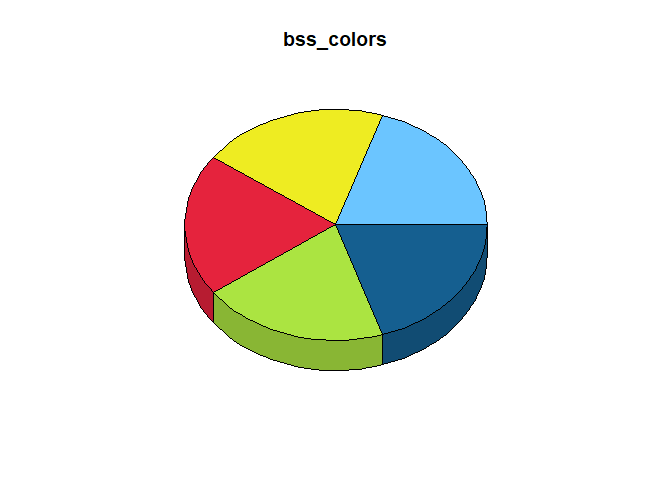
\includegraphics[width=1\linewidth]{man/figures/README-unnamed-chunk-2-1}

\begin{Shaded}
\begin{Highlighting}[]
\CommentTok{\#hashes \textless{}{-} bss\_colors$hashed\_hex}
\NormalTok{bss\_colors }\OtherTok{\textless{}{-}}\NormalTok{ bss\_colors[}\FunctionTok{order}\NormalTok{(bss\_colors}\SpecialCharTok{$}\NormalTok{col\_pal),] }

\FunctionTok{swatch}\NormalTok{(bss\_colors}\SpecialCharTok{$}\NormalTok{hashed\_hex)}
\end{Highlighting}
\end{Shaded}

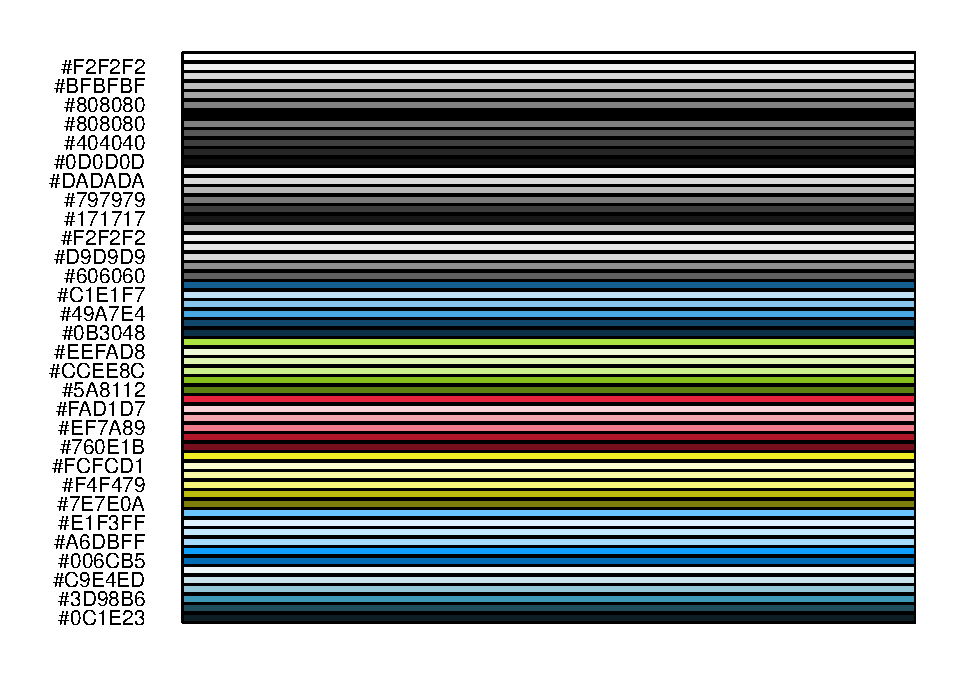
\includegraphics[width=1\linewidth]{man/figures/README-unnamed-chunk-2-2}

\begin{Shaded}
\begin{Highlighting}[]
\NormalTok{choice }\OtherTok{\textless{}{-}}\NormalTok{ bss\_colors }\SpecialCharTok{\%\textgreater{}\%} \FunctionTok{filter}\NormalTok{(col\_pal }\SpecialCharTok{==} \DecValTok{7}\NormalTok{) }
\FunctionTok{swatch}\NormalTok{(choice}\SpecialCharTok{$}\NormalTok{hashed\_hex)}
\end{Highlighting}
\end{Shaded}

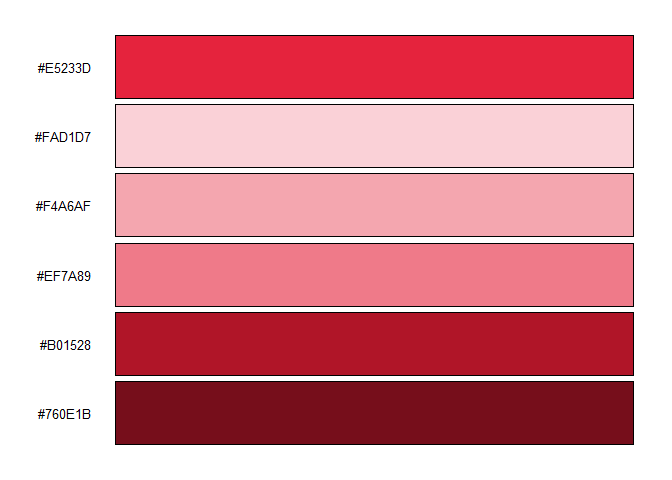
\includegraphics[width=1\linewidth]{man/figures/README-unnamed-chunk-2-3}

\begin{Shaded}
\begin{Highlighting}[]
\FunctionTok{swatch}\NormalTok{(basic\_colors)}
\end{Highlighting}
\end{Shaded}

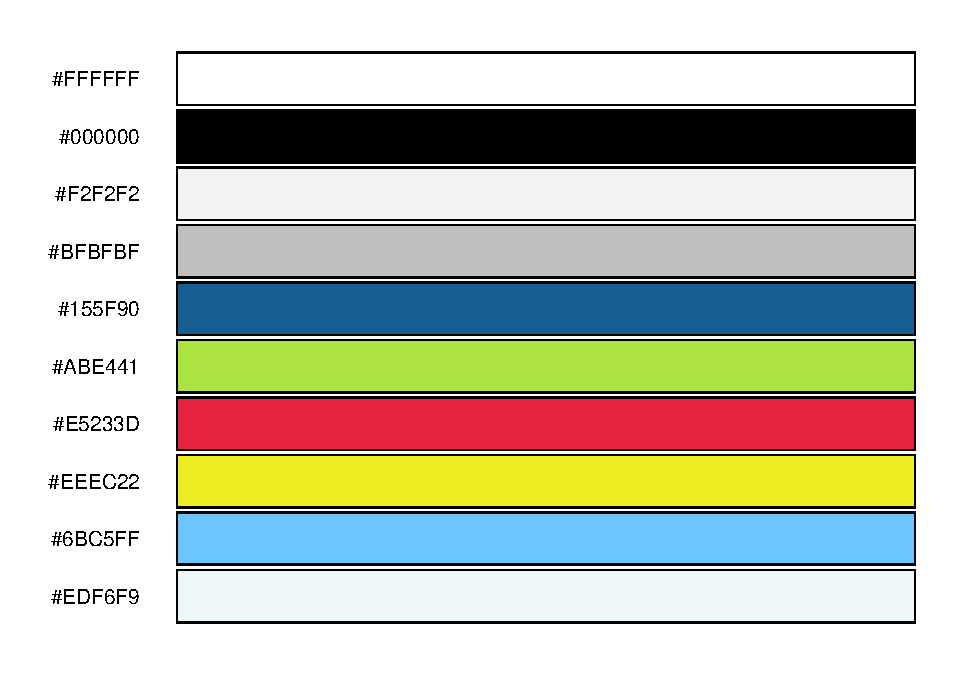
\includegraphics[width=1\linewidth]{man/figures/README-unnamed-chunk-2-4}

\hypertarget{function-bss_cols---examples}{%
\subsection{function: bss\_cols() -
examples}\label{function-bss_cols---examples}}

The bss\_cols function allows you to get and reference hex colors in a
robust and flexible way.

\begin{Shaded}
\begin{Highlighting}[]
\CommentTok{\# to get the information of a color}
\FunctionTok{bss\_cols}\NormalTok{(}\StringTok{"rot"}\NormalTok{)}
\CommentTok{\#\textgreater{}       rot }
\CommentTok{\#\textgreater{} "\#E5233D"}
\CommentTok{\# or to just use a color in a plot}
\FunctionTok{ggplot}\NormalTok{(mtcars, }\FunctionTok{aes}\NormalTok{(hp, mpg)) }\SpecialCharTok{+}
  \FunctionTok{geom\_point}\NormalTok{(}\AttributeTok{color =} \FunctionTok{bss\_cols}\NormalTok{(}\StringTok{"rot"}\NormalTok{),}
             \AttributeTok{size =} \DecValTok{2}\NormalTok{, }\AttributeTok{alpha =}\NormalTok{ .}\DecValTok{8}\NormalTok{)}
\end{Highlighting}
\end{Shaded}

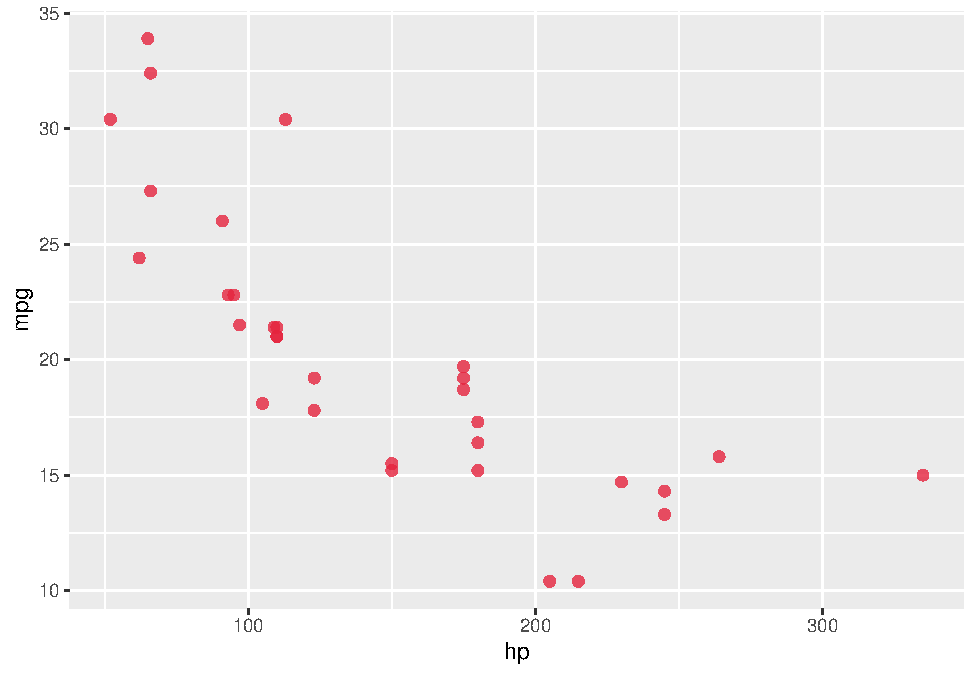
\includegraphics[width=1\linewidth]{man/figures/README-bss_cols-1}

\hypertarget{function-bss_pal---examples}{%
\subsection{function: bss\_pal() -
examples}\label{function-bss_pal---examples}}

With a subset of palettes of the original colors this function allows to
interpolate the palette colors for a certain number of levels, making it
possible to create shades between the original colors using
colorRampPalette from grDevices. Further, it gets a palette by name from
the list (``main'' by default) and has a boolean condition determining
whether to reverse the order or not.

\begin{Shaded}
\begin{Highlighting}[]
\CommentTok{\# the following subset color palettes are available }
\NormalTok{bss\_palettes}
\CommentTok{\#\textgreater{} $monochrom\_black1}
\CommentTok{\#\textgreater{}            [,1]      [,2]      [,3]      [,4]      [,5]      [,6]     }
\CommentTok{\#\textgreater{} hashed\_hex "\#FFFFFF" "\#F2F2F2" "\#D9D9D9" "\#BFBFBF" "\#A6A6A6" "\#808080"}
\CommentTok{\#\textgreater{} }
\CommentTok{\#\textgreater{} $monochrom\_green}
\CommentTok{\#\textgreater{}            [,1]      [,2]      [,3]      [,4]      [,5]      [,6]     }
\CommentTok{\#\textgreater{} hashed\_hex "\#ABE441" "\#EEFAD8" "\#DDF4B3" "\#CCEE8C" "\#86BF1C" "\#5A8112"}
\CommentTok{\#\textgreater{} }
\CommentTok{\#\textgreater{} $monochrom\_red}
\CommentTok{\#\textgreater{}            [,1]      [,2]      [,3]      [,4]      [,5]      [,6]     }
\CommentTok{\#\textgreater{} hashed\_hex "\#E5233D" "\#FAD1D7" "\#F4A6AF" "\#EF7A89" "\#B01528" "\#760E1B"}
\CommentTok{\#\textgreater{} }
\CommentTok{\#\textgreater{} $monochrom\_yellow}
\CommentTok{\#\textgreater{}            [,1]      [,2]      [,3]      [,4]      [,5]      [,6]     }
\CommentTok{\#\textgreater{} hashed\_hex "\#EEEC22" "\#FCFCD1" "\#F9F9A6" "\#F4F479" "\#BDBD0F" "\#7E7E0A"}
\CommentTok{\#\textgreater{} }
\CommentTok{\#\textgreater{} $monochrom\_blue}
\CommentTok{\#\textgreater{}            [,1]      [,2]      [,3]      [,4]      [,5]      [,6]     }
\CommentTok{\#\textgreater{} hashed\_hex "\#6BC5FF" "\#E1F3FF" "\#C4E8FF" "\#A6DBFF" "\#0F9FFF" "\#006CB5"}
\CommentTok{\#\textgreater{} }
\CommentTok{\#\textgreater{} $main}
\CommentTok{\#\textgreater{}            [,1]      [,2]      [,3]      [,4]      [,5]      [,6]     }
\CommentTok{\#\textgreater{} hashed\_hex "\#FFFFFF" "\#000000" "\#F2F2F2" "\#BFBFBF" "\#155F90" "\#ABE441"}
\CommentTok{\#\textgreater{}            [,7]      [,8]      [,9]      [,10]    }
\CommentTok{\#\textgreater{} hashed\_hex "\#E5233D" "\#EEEC22" "\#6BC5FF" "\#EDF6F9"}
\CommentTok{\#\textgreater{} }
\CommentTok{\#\textgreater{} $main\_only\_color}
\CommentTok{\#\textgreater{}            [,1]      [,2]      [,3]      [,4]      [,5]     }
\CommentTok{\#\textgreater{} hashed\_hex "\#155F90" "\#ABE441" "\#E5233D" "\#EEEC22" "\#6BC5FF"}

\CommentTok{\# interpolate the "rgb" palette (which only includes three colors, red, green and blue) to a length of 9:}
\FunctionTok{bss\_pal}\NormalTok{(}\StringTok{"main\_only\_color"}\NormalTok{)(}\DecValTok{5}\NormalTok{)}
\CommentTok{\#\textgreater{} [1] "\#155F90" "\#ABE441" "\#E5233D" "\#EEEC22" "\#6BC5FF"}
\FunctionTok{pie3D}\NormalTok{(}\FunctionTok{rep}\NormalTok{(}\DecValTok{5}\NormalTok{, }\DecValTok{6}\NormalTok{),}\AttributeTok{explode=}\DecValTok{0}\NormalTok{, }\AttributeTok{theta=}\FloatTok{1.2}\NormalTok{, }\AttributeTok{col=}\FunctionTok{bss\_pal}\NormalTok{(}\StringTok{"monochrom\_yellow"}\NormalTok{)(}\DecValTok{6}\NormalTok{), }\AttributeTok{main=}\StringTok{"bss\_pal(\textquotesingle{}monochrom\_yellow\textquotesingle{})(6)"}\NormalTok{)}
\end{Highlighting}
\end{Shaded}

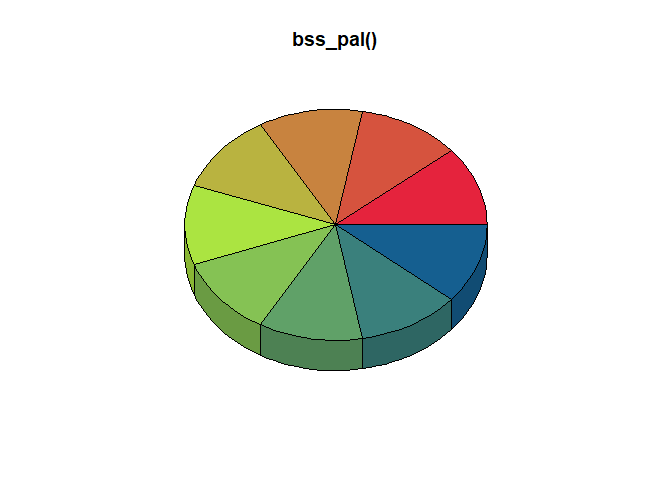
\includegraphics[width=1\linewidth]{man/figures/README-bss_pal-1}

\hypertarget{function-scale_color_bss---example}{%
\subsection{function: scale\_color\_bss() -
example}\label{function-scale_color_bss---example}}

Custom color scale functions for ggplot2.

\begin{Shaded}
\begin{Highlighting}[]
\CommentTok{\# Color by discrete variable using default palette}
\FunctionTok{ggplot}\NormalTok{(iris, }\FunctionTok{aes}\NormalTok{(Sepal.Width, Sepal.Length, }\AttributeTok{color =}\NormalTok{ Species)) }\SpecialCharTok{+}
  \FunctionTok{geom\_point}\NormalTok{(}\AttributeTok{size =} \DecValTok{2}\NormalTok{) }\SpecialCharTok{+}
  \FunctionTok{scale\_color\_bss}\NormalTok{()}
\end{Highlighting}
\end{Shaded}

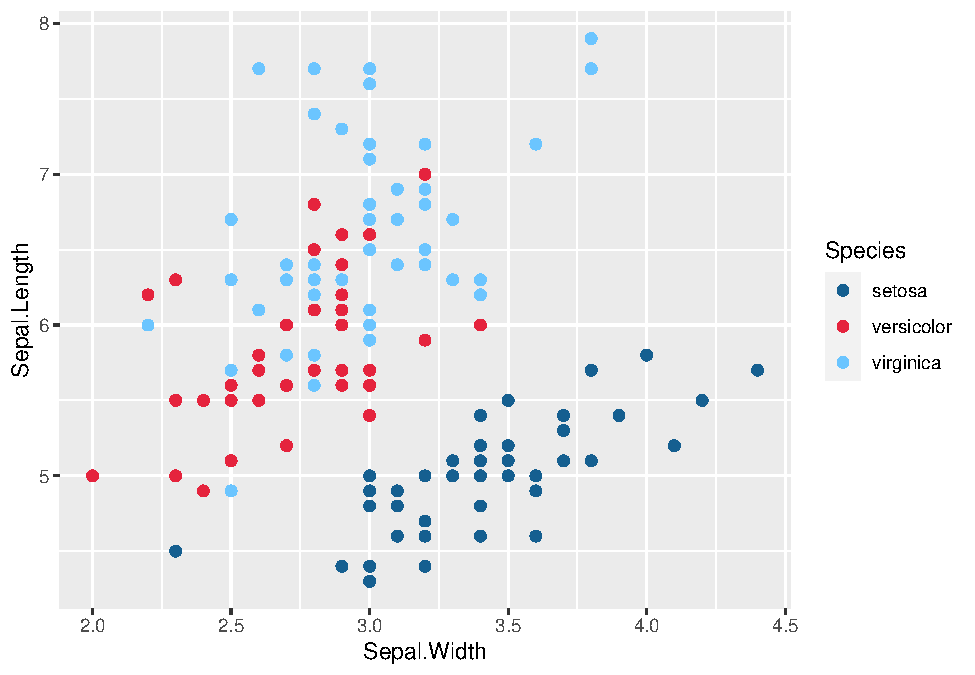
\includegraphics[width=1\linewidth]{man/figures/README-scale_color_bss-1}

\begin{Shaded}
\begin{Highlighting}[]

\CommentTok{\# Color by numeric variable with cool palette}
\FunctionTok{ggplot}\NormalTok{(iris, }\FunctionTok{aes}\NormalTok{(Sepal.Width, Sepal.Length, }\AttributeTok{color =}\NormalTok{ Sepal.Length)) }\SpecialCharTok{+}
  \FunctionTok{geom\_point}\NormalTok{(}\AttributeTok{size =} \DecValTok{2}\NormalTok{, }\AttributeTok{alpha =}\NormalTok{ .}\DecValTok{6}\NormalTok{) }\SpecialCharTok{+}
  \FunctionTok{scale\_color\_bss}\NormalTok{(}\AttributeTok{discrete =} \ConstantTok{FALSE}\NormalTok{, }\AttributeTok{palette =} \StringTok{"monochrom\_red"}\NormalTok{)}
\end{Highlighting}
\end{Shaded}

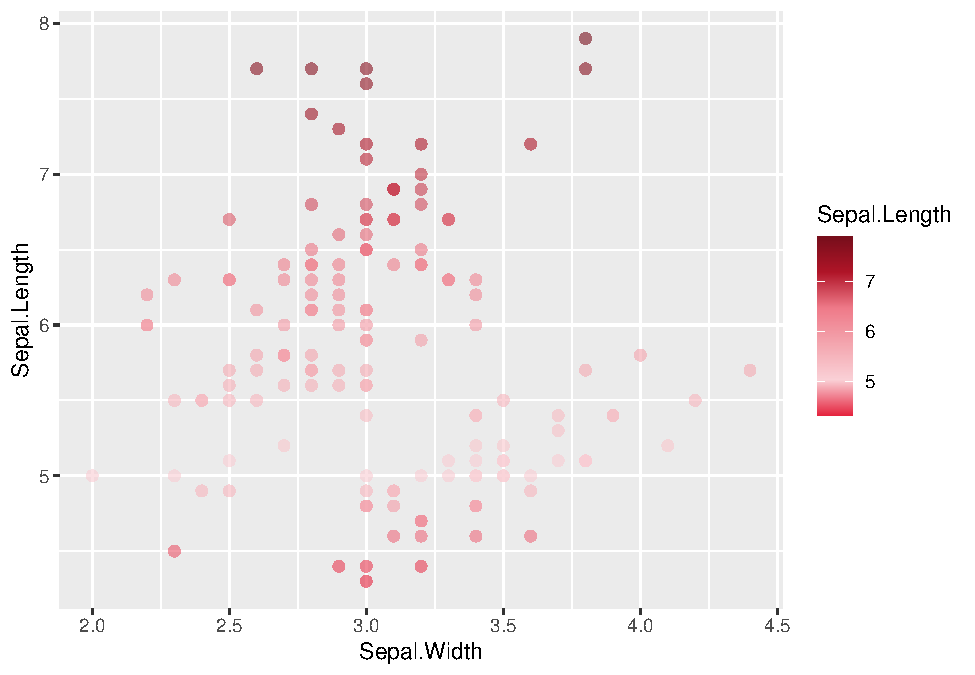
\includegraphics[width=1\linewidth]{man/figures/README-scale_color_bss-2}

\hypertarget{function-scale_fill_bss---example}{%
\subsection{function: scale\_fill\_bss() -
example}\label{function-scale_fill_bss---example}}

Custom fill scale functions for ggplot2.

\begin{Shaded}
\begin{Highlighting}[]
\CommentTok{\# Fill by discrete variable with different palette + remove legend (guide)}
\FunctionTok{ggplot}\NormalTok{(mpg, }\FunctionTok{aes}\NormalTok{(model          , }\AttributeTok{fill =}\NormalTok{ model         )) }\SpecialCharTok{+}
  \FunctionTok{geom\_bar}\NormalTok{() }\SpecialCharTok{+}
  \FunctionTok{theme}\NormalTok{(}\AttributeTok{axis.text.x =} \FunctionTok{element\_text}\NormalTok{(}\AttributeTok{angle =} \DecValTok{45}\NormalTok{, }\AttributeTok{hjust =} \DecValTok{1}\NormalTok{)) }\SpecialCharTok{+}
  \FunctionTok{scale\_fill\_bss}\NormalTok{(}\AttributeTok{palette =} \StringTok{"main"}\NormalTok{, }\AttributeTok{guide =} \StringTok{"none"}\NormalTok{)}
\end{Highlighting}
\end{Shaded}

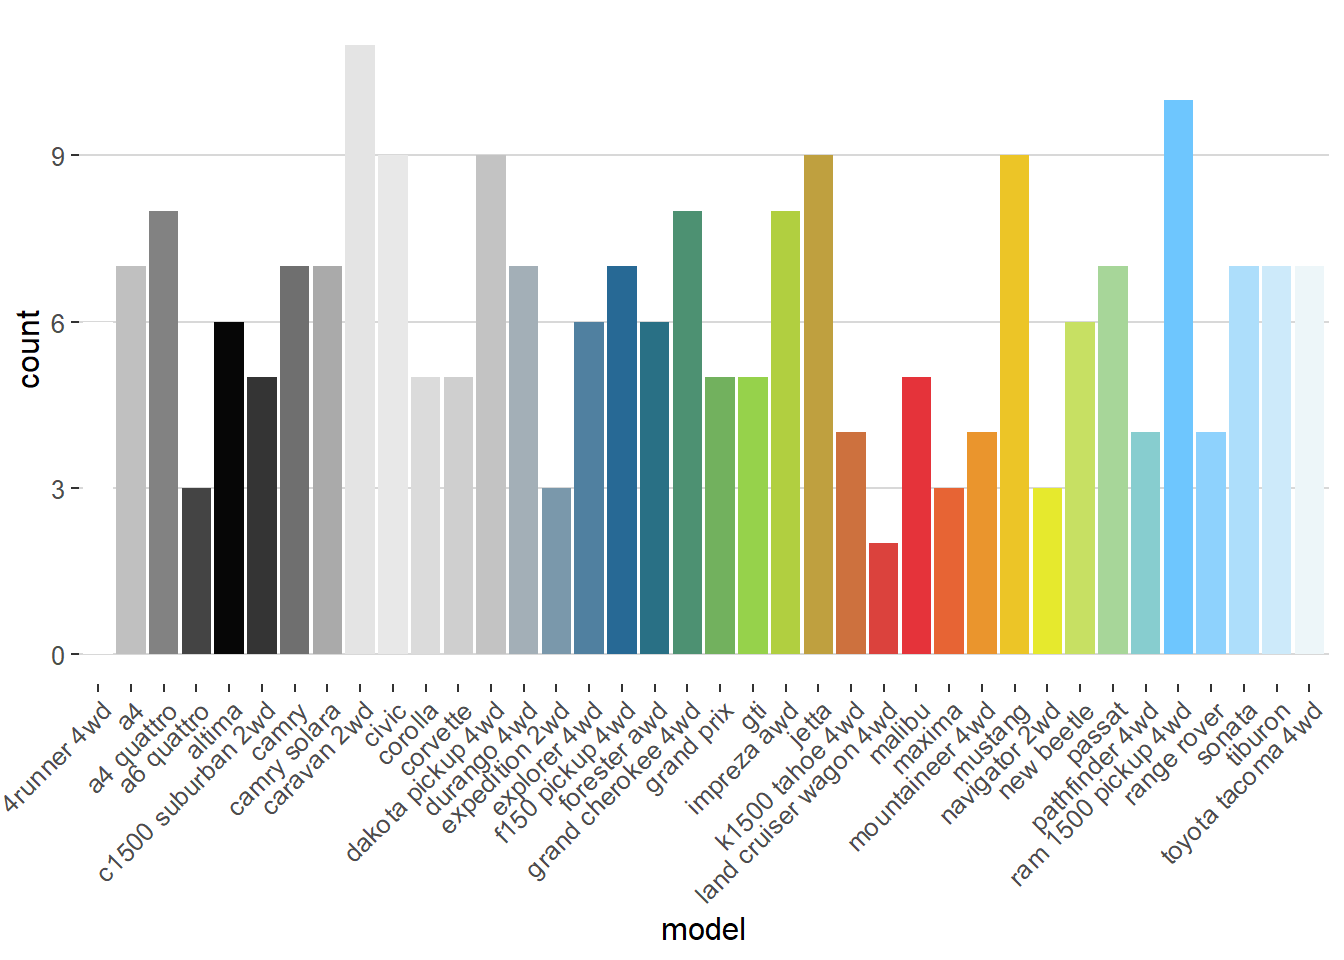
\includegraphics[width=1\linewidth]{man/figures/README-scale_fill_bss-1}

\end{document}
